%da https://blog.angular-university.io/service-workers/ e https://developer.mozilla.org/en-US/docs/Web/API/Service_Worker_API
\documentclass[italian]{article}
\usepackage[T1]{fontenc}
\usepackage[utf8]{inputenc}
\usepackage{lmodern}
\usepackage{hyperref}
\usepackage[a4paper,top=3cm,bottom=3cm,left=2.5cm,right=2.5cm]{geometry}
\usepackage[italian]{babel}
\usepackage{listings} %Per inserire codice
\usepackage[usenames]{color} %Per permettere la colorazione dei caratteri 
%Define the listing package
\usepackage{listings} %code highlighter
\usepackage{color} %use color
\usepackage{graphicx}
\graphicspath{ {./images/} }
\definecolor{mygreen}{rgb}{0,0.6,0}
\definecolor{mygray}{rgb}{0.5,0.5,0.5}
\definecolor{mymauve}{rgb}{0.58,0,0.82}

%Customize a bit the look
\lstset{ %
	backgroundcolor=\color{white}, % choose the background color; you must add \usepackage{color} or \usepackage{xcolor}
	basicstyle=\footnotesize, % the size of the fonts that are used for the code
	breakatwhitespace=false, % sets if automatic breaks should only happen at whitespace
	breaklines=true, % sets automatic line breaking
	captionpos=b, % sets the caption-position to bottom
	commentstyle=\color{mygreen}, % comment style
	deletekeywords={...}, % if you want to delete keywords from the given language
	escapeinside={\%*}{*)}, % if you want to add LaTeX within your code
	extendedchars=true, % lets you use non-ASCII characters; for 8-bits encodings only, does not work with UTF-8
	frame=single, % adds a frame around the code
	keepspaces=true, % keeps spaces in text, useful for keeping indentation of code (possibly needs columns=flexible)
	keywordstyle=\color{blue}, % keyword style
	% language=Octave, % the language of the code
	morekeywords={*,...}, % if you want to add more keywords to the set
	numbers=left, % where to put the line-numbers; possible values are (none, left, right)
	numbersep=5pt, % how far the line-numbers are from the code
	numberstyle=\tiny\color{mygray}, % the style that is used for the line-numbers
	rulecolor=\color{black}, % if not set, the frame-color may be changed on line-breaks within not-black text (e.g. comments (green here))
	showspaces=false, % show spaces everywhere adding particular underscores; it overrides 'showstringspaces'
	showstringspaces=false, % underline spaces within strings only
	showtabs=false, % show tabs within strings adding particular underscores
	stepnumber=1, % the step between two line-numbers. If it's 1, each line will be numbered
	stringstyle=\color{mymauve}, % string literal style
	tabsize=2, % sets default tabsize to 2 spaces
	title=\lstname % show the filename of files included with \lstinputlisting; also try caption instead of title
}
%END of listing package%

\definecolor{darkgray}{rgb}{.4,.4,.4}
\definecolor{purple}{rgb}{0.65, 0.12, 0.82}

%define Javascript language
\lstdefinelanguage{JavaScript}{
	keywords={typeof, new, true, false, catch, function, return, null, catch, switch, var, if, in, while, do, else, case, break},
	keywordstyle=\color{blue}\bfseries,
	ndkeywords={class, export, boolean, throw, implements, import, this},
	ndkeywordstyle=\color{darkgray}\bfseries,
	identifierstyle=\color{black},
	sensitive=false,
	comment=[l]{//},
	morecomment=[s]{/*}{*/},
	commentstyle=\color{purple}\ttfamily,
	stringstyle=\color{red}\ttfamily,
	morestring=[b]',
	morestring=[b]"
}

\lstset{
	language=JavaScript,
	extendedchars=true,
	basicstyle=\footnotesize\ttfamily,
	showstringspaces=false,
	showspaces=false,
	numbers=left,
	numberstyle=\footnotesize,
	numbersep=9pt,
	tabsize=2,
	breaklines=true,
	showtabs=false,
	captionpos=b
}
\author{
	Daniele Rigon - 857319 \\
}

\begin{document}
\title{Tesi - Payment Request API}
\maketitle

\tableofcontents
\pagebreak

\section{Overview}
Un service worker è uno script Javascript, che utilizza gli oggetti Promise per poter eseguire operazioni in modalità asincrona (quindi non bloccanti), che il browser avvia in background separato dalla pagina, pertanto non può modificarne gli elementi come i normali script (non ha accesso al DOM) ma può comunicare con essi mediante “messaggi”.

Un Service Worker si trova tra la nostra applicazione Web e la rete e, come un server proxy, può intercettare tutte le richieste a pagine web e file statici e rispondere secondo politiche che siamo noi stessi a decidere.

I service worker sono pensati per consentire la creazione di esperienze offline efficaci, intercettare le richieste di rete e intraprendere azioni appropriate in base al fatto che la rete sia disponibile o meno e aggiornare le risorse che risiedono sul server, oltre a consentire l'accesso alle notifiche push e alle API di sincronizzazione in background.

È il browser che in qualsiasi momento deciderà se il Service Worker dovrebbe essere o meno in esecuzione: questo per risparmiare risorse, specialmente sui dispositivi mobili. Per questo può essere che se non facciamo alcuna richiesta HTTP per un certo periodo di tempo o non riceviamo alcuna notifica per un po' è possibile che il browser spenga il Service Worker. Se attiviamo una richiesta HTTP che deve essere gestita dal Service Worker, il browser la attiverà di nuovo, nel caso in cui non fosse ancora in esecuzione. Quindi vedere il Service Worker bloccato in Dev Tools non significa necessariamente che qualcosa è rotto o non va.

\subsection{Impostare i service worker}
Molte funzionalità dei Service Worker oggi sono abilitate di default nelle versioni più recenti dei browser. Se il codice demo seguente non funziona bisogna abilitare un pref:
\begin{itemize}
	\item Firefox: su \url{about:config} impostare dom.serviceWorkers.enabled su true; riavvia il browser.
	\item Chrome : su \url{chrome://flags} accendere  experimental-web-platform-features; riavvia browser
	\item Opera : su \url{opera://flags} attivare Support for ServiceWorker; riavvia il browser.
	\item Microsoft Edge : su \url{about:flags} spuntare  Enable service workers; riavvia il browser.
\end{itemize}

\section{Architettura di base}
Per quanto riguarda i Service Worker generalmente vengono eseguiti questi passaggi per l'impostazione di base:
\begin{itemize}
	\item L'URL del Service Worker viene recuperato e registrato tramite serviceWorkerContainer.register();
	\item In caso di esito positivo, il Service Worker viene eseguito in un ServiceWorkerGlobalScope, ovvero un tipo speciale di Service Context che scappa dal thread di esecuzione dello script principale senza accesso DOM.
	\item Il Service Worker ora è pronto per elaborare gli eventi;
	\item L'installazione del Service Worker viene tentata quando si accede successivamente alle pagine. Un evento di installazione è sempre il primo inviato a un Service Worker;
	\item Quando il Service Worker  è considerato installato, il passo successivo è l'attivazione; quindi quando il Service Worker è installato riceve un evento di attivazione. L'uso principale di onactivate è per la pulizia delle risorse utilizzate nelle versioni precedenti di uno script di servizio.
\end{itemize}
\begin{figure}[h]
	\centering
	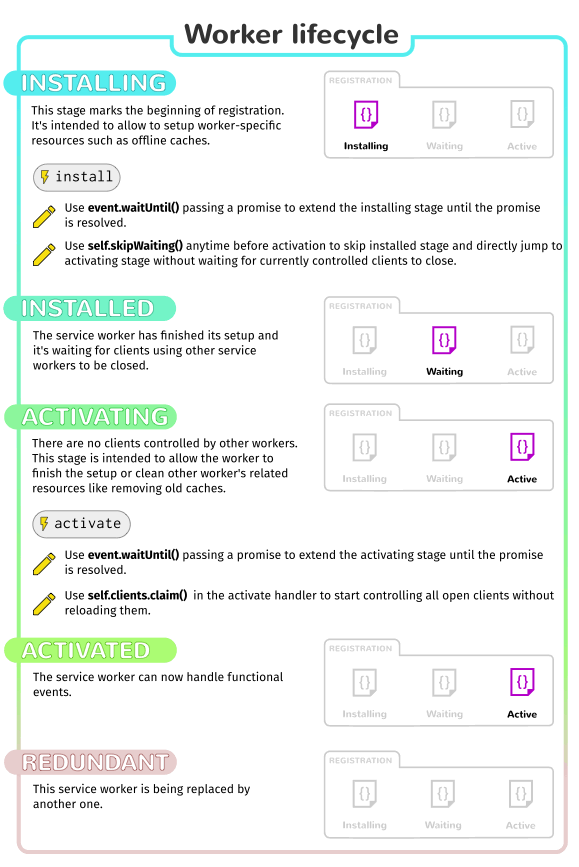
\includegraphics[width=0.6\linewidth]{SwLifecycle}
	\caption{Ciclo di vita del Service Worker}
	\label{fig:Ciclo di vita del Service Worker}
\end{figure}
\pagebreak
\newpage

\subsection{Casi d'uso}
I Service Worker sono anche destinati a essere utilizzati per cose come:
\begin{itemize}
	\item Sincronizzazione dei dati in background;
	\item Rispondere alle richieste di risorse da altre origini;
	\item Ricezione di aggiornamenti centralizzati a dati costosi da calcolare in modo che più pagine possano utilizzare un set di dati;
	\item Modelli personalizzati basati su determinati pattern URL;
	\item Miglioramenti delle prestazioni, ad esempio prelettura delle risorse che l'utente probabilmente avrà bisogno nel prossimo futuro.
\end{itemize}
Altre specifiche sono utilizzate dal Service Context, ad esempio:
\begin{itemize}
	\item Sincronizzazione in background : avvia un operatore di servizio anche quando nessun utente si trova sul sito, quindi le cache possono essere aggiornate, ecc;
	\item Reagire per inviare messaggi : si può avviare un Service Worker per inviare agli utenti un messaggio per comunicare loro che sono disponibili nuovi contenuti;
	\item Reagendo ad orari e date particolari.
\end{itemize}

\section{Ciclo di vita di un Service Worker}
Il ciclo di vita di un service worker è composto da quattro fasi:
\begin{itemize}
\item Registrazione: il service worker viene scaricato dal browser, analizzato ed eseguito;
\item Installazione: il service worker viene installato;
\item Attivazione: il service worker è pronto ed è in grado di poter controllare gli eventi generati dal client;
\item Fetch: evento generato dal client. Il service worker è in grado di intercettare le richieste e rispondere secondo le opportune strategie di caching. 
\end{itemize}

\subsection{Registrazione}

Come prima cosa bisogna comunicare al browser l’esistenza di un service worker all’interno del sito web. Un Service Worker viene prima registrato utilizzando il metodo ServiceWorker.register(), e per farlo basta inserire su tutte le pagine del sito uno script come il seguente:
\begin{lstlisting}
if ('serviceWorker' in navigator) { // Path che contiene il service worker navigator.serviceWorker.register('/service-worker.js').then(function(registration) { console.log('Service worker installato correttamente, ecco lo scope:', registration.scope); }).catch(function(error) { console.log('Installazione service worker fallita:', error); });
}
\end{lstlisting}
Il codice inizia controllando il supporto da parte del browser verificando la presenza di navigator.serviceWorker. Se supportato il service worker viene registrato per mezzo di navigator.serviceWorker.register che restituisce un oggetto Promise il quale si risolve con successo a registrazione avvenuta correttamente.
service-worker.js è il file Javascript residente nella root del sito web e che contiene il codice del service worker, il cui codice è:
\begin{lstlisting}
// Evento install
self.addEventListener('install', event => { // Codice da eseguire su installazione console.log("Service Worker Installato");
});
// Evento activate
self.addEventListener('activate', event => { // Codice da eseguire su attivazione console.log("Service Worker Attivo");
});
// Evento fetch
self.addEventListener('fetch', event => { // Codice da eseguire su fetch di risorse console.log("Richiesta URL: "+event.request.url);
});
\end{lstlisting}

In questo modo viene registrato un Service Worker il quale al momento non fa nulla di interessante, viene semplicemente installato e ad ogni richiesta stampa in console un messaggio con la URL che il browser tenta di scaricare dal server web. Per controllare il caricamento di un Service Worker il codice di questo deve essere eseguito al di fuori delle normali pagine.

Possono esserci diversi motivi per cui il Service Worker non si registra:
\begin{itemize}
	\item Non si sta eseguendo l'applicazione tramite HTTPS;
	\item Il path del Service Worker non è scritto correttamente: deve essere scritto in relazione all'origine, non alla directory radice dell'app;
	\item Il Service Worker a cui ci si riferisce ha un'origine diversa da quella della tua app.
\end{itemize}

\subsection{Installazione}
Il Service Worker viene scaricato immediatamente quando un utente accede per la prima volta a un sito, o una pagina, controllata dal Service Worker, e sarà poi scaricato periodicamente ogni tot periodo di tempo.

L'installazione viene tentata quando il file nuovo che è stato scaricato risulta diverso da un Service Worker esistente, o risulta essere diverso dal primo Service Worker rilevato per quella pagina/sito. Se è la prima volta che un Service Worker viene reso disponibile viene tentata l'installazione e, dopo un'installazione corretta, viene attivato. Se è disponibile un Service Worker esistente, la nuova versione viene installata in background, ma non ancora attivata; si attiva solo quando non ci sono più pagine caricate che stanno ancora utilizzando il vecchio Service Worker. Non appena non ci sono più pagine da caricare, il nuovo Service Worker si attiva.

Conseguentemente all’installazione viene richiamato l’evento install. Tale evento consente di effettuare il precaching, ovvero inserire in cache pagine e file statici del sito web prima di intercettarne le richieste. Per farlo occorre utilizzare gli oggetti Promise event e cache come segue:
\begin{lstlisting}
	'use strict';
	// Array di configurazione del service worker
	var config = {
	version: 'versionesw1::',
	// Risorse da inserire in cache immediatamente - Precaching
	staticCacheItems: [ '/wp-includes/js/jquery/jquery.js', '/wp-content/themes/miotema/logo.png', '/wp-content/themes/miotema/fonts/opensans.woff', '/wp-content/themes/miotema/fonts/fontawesome-webfont.woff2',
	],
	};
	// Funzione che restituisce una stringa da utilizzare come chiave per la cache
	function cacheName (key, opts) { return `${opts.version}${key}`;
	}
	// Evento install
	self.addEventListener('install', event => { event.waitUntil( // Inserisco in cache le URL configurate in config.staticCacheItems caches.open( cacheName('static', config) ).then(cache => cache.addAll(config.staticCacheItems)) // self.skipWaiting() evita l'attesa, il che significa che il service worker si attivera immediatamente non appena conclusa l'installazione .then( () => self.skipWaiting() ) ); console.log("Service Worker Installato");
	});
\end{lstlisting}
Se si decidesse di aggiungere/eliminare nuove risorse da inserire in cache, bisognerà avere l’accortezza di cambiare il nome della versione del service worker ed eliminare dalla cache le risorse già presenti.
Una cosa molto importante da sapere è che le risorse da inserire in cache in fase di precaching devono esistere realmente sul server web altrimenti il service worker genererà un errore fatale e l’installazione non andrà a buon fine. 
Il metodo skipWaiting() consente al service worker di passare allo stato di attivazione ad installazione conclusa e quindi essere subito operativo.

\subsection{Attivazione}
Una volta installato, il service worker passa nello stato di attivazione. Se la pagina al momento è controllata da un altro service worker, l’attuale passa in uno stato di attesa per poi diventare operativo al prossimo caricamento di pagina, quando il vecchio service worker viene sostituito.

Questo per essere sicuri che solo un service worker (o una sola versione di service worker) per volta possa essere eseguito nello stesso contesto temporale.

A service worker attivato, viene richiamato l’evento activate, l’evento ideale per svuotare la cache obsoleta dell’eventuale precedente versione di service worker. Dopodiché il service worker sarà in grado di effettuare fetching di risorse o restare in attesa di altri eventi.

Di default il nuovo service worker diventa operativo al refresh della pagina o dopo aver richiamato il metodo clients.claim(). Fino a quel momento le eventuali richieste non saranno intercettate. 

Di seguito un codice di esempio eseguito al verificarsi dell’evento activate. Il codice effettua il purge della cache di versioni del service worker diverse dall’attuale e successivamente  richiama clients.claim() per poter intercettare le richieste fin da subito.

\begin{lstlisting}
	self.addEventListener('activate', event => { // Questa funzione elimina dalla cache tutte le risorse la cui chiave non contiene il nome della versione // impostata sul config di questo service worker function clearCacheIfDifferent(event, opts) { return caches.keys().then(cacheKeys => { var oldCacheKeys = cacheKeys.filter(key => key.indexOf(opts.version) !== 0); var deletePromises = oldCacheKeys.map(oldKey => caches.delete(oldKey)); return Promise.all(deletePromises); }); }
	event.waitUntil( // Se la versione del service worker cambia, svuoto la cache clearCacheIfDifferent(event, config) // Con self.clients.claim() consento al service worker di poter intercettare le richieste (fetch) fin da subito piuttosto che attendere il refresh della pagina .then( () => self.clients.claim() ) ); console.log("Service Worker Avviato");
	});
\end{lstlisting}

\subsection{Fetch}
Grazie all’evento fetch il service worker potrà agire da proxy tra l’applicazione web e la rete.

Il service worker intercetterà ogni richiesta HTTP del browser e sarà in grado di rispondere a quest’ultimo prendendo la risorsa dalla cache piuttosto che scaricarla dalla rete o applicando le più disparate strategie di caching.

Grazie all’evento fetch il service worker diventa un vero e proprio strumento per migliorare le performance di caricamento di un sito web.


\subsection{Aggiornare il Service Worker}
Se il Service Worker è già stato installato, ma una nuova versione è disponibile per l'aggiornamento o il caricamento della pagina, la nuova versione viene installata in background ma non sarà ancora attivata. Si attiva solo quando non ci sono più pagine caricate che stanno ancora utilizzando il vecchio servizio. Non appena non ci sono più pagine di questo tipo ancora caricate, il nuovo Service Worker si attiverà.

Si dovrà aggiornare il listener install di eventi nel nuovo Service Worker, similmente a questo:
\begin{lstlisting}
self.addEventListener('install', function(event) {
	event.waitUntil(
		caches.open('v2').then(function(cache) {
			return cache.addAll([
				'/sw-test/',
				'/sw-test/index.html',
				'/sw-test/style.css',
				'/sw-test/app.js',
				'/sw-test/image-list.js',
								
				// include other new resources for the new version...
			]);
		})
	);
});
\end{lstlisting}
Mentre accade questo è ancora la versione precedente (v1) quella responsabile per i recuperi, mentre la nuova versione (v2) si sta installando in background.
Quando nessuna pagina sta utilizzando la versione corrente, il nuovo operatore si attiva e diventa responsabile dei recuperi.

\subsection{Disintallare il Service Worker}

Rimuovere/disinstallare un service worker è un’operazione piuttosto semplice. È possibile eseguirla manualmente dal proprio browser oppure inserendo un semplice script al posto di quello di registrazione del service worker:

\begin{lstlisting}
	navigator.serviceWorker.getRegistrations().then(function(registrations) { for(let registration of registrations) { registration.unregister() }
	})
\end{lstlisting}
Naturalmente è necessario che la pagina contenente il codice di disinstallazione venga visitata dal browser. È possibile procedere anche alla rimozione manuale su Google Chrome semplicemente aprendo la DevTools e cliccando prima su Application e successivamente su Service Workers. Accanto al service worker sarà presente un link dal nome Unregister. Non resta che cliccarci sopra per disinstallare e rimuovere il service worker in via definitiva.

\section{Compatibilità web}
\subsection{Desktop}
\begin{figure}[h]
	\centering
	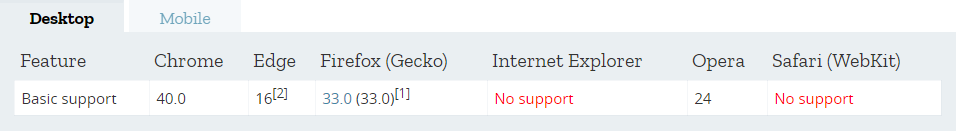
\includegraphics[width=1\linewidth]{CompWeb}
	\caption{Compatibilità web}
	\label{fig:Compatibilità web}
\end{figure}
\subsection{Mobile}
\begin{figure}[h]
	\centering
	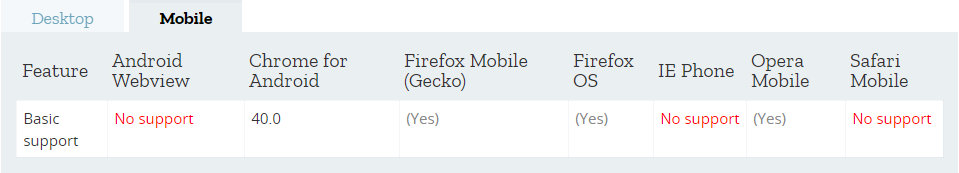
\includegraphics[width=1\linewidth]{CompMobile}
	\caption{Compatibilità mobile}
	\label{fig:Compatibilità mobile}
\end{figure}

\section{Conclusioni}
Se realizzati da un esperto i service worker possono rendere la navigazione del sito web molto ma molto veloce. Grazie alla loro implementazione esterna, non richiedono modifica alcuna al sito web, motivo per cui sono molto apprezzati nel ramo delle web performance.
\end{document}